\documentclass[tikz]{standalone}
\usepackage{graphicx}
\usepackage{adjustbox}
\usepackage{subcaption}
\usepackage{caption}
\usepackage{comment}
\usepackage{tikz}
\usepackage{textcomp}
\usetikzlibrary {arrows.meta,bending,positioning}

\definecolor{Okabe1}{RGB}{000,158,115}
\definecolor{Okabe2}{RGB}{000,114,178}
\definecolor{Okabe3}{RGB}{086,180,233}
\definecolor{Okabe4}{RGB}{230,159,000}
\definecolor{Okabe5}{RGB}{213,094,000}
\definecolor{Okabe6}{RGB}{204,121,167}

\definecolor{b1}{HTML}{d73027}
\definecolor{b2}{HTML}{fc8d59}
\definecolor{b3}{HTML}{ffffbf}
\definecolor{b4}{HTML}{91bfdb}
\definecolor{b5}{HTML}{4575b4}

\begin{document}
	\begin{comment}
		\begin{tabular}{@{}c@{}c@{}}
			\includegraphics[width=0.5\textwidth]{shellAmbient.jpg} &
			\includegraphics[width=0.5\textwidth]{shellCrushed.jpg} \\
			\noalign{\vskip -4pt}
			\includegraphics[width=0.5\textwidth]{shellNeg.jpg} &
			\includegraphics[width=0.5\textwidth]{shellHold.jpg}
		\end{tabular}.
	\end{comment}
	\begin{tikzpicture}
		\tikzstyle{every node}=[font=\LARGE]
		
		\node[anchor=north west,inner sep=0] at (0,0) {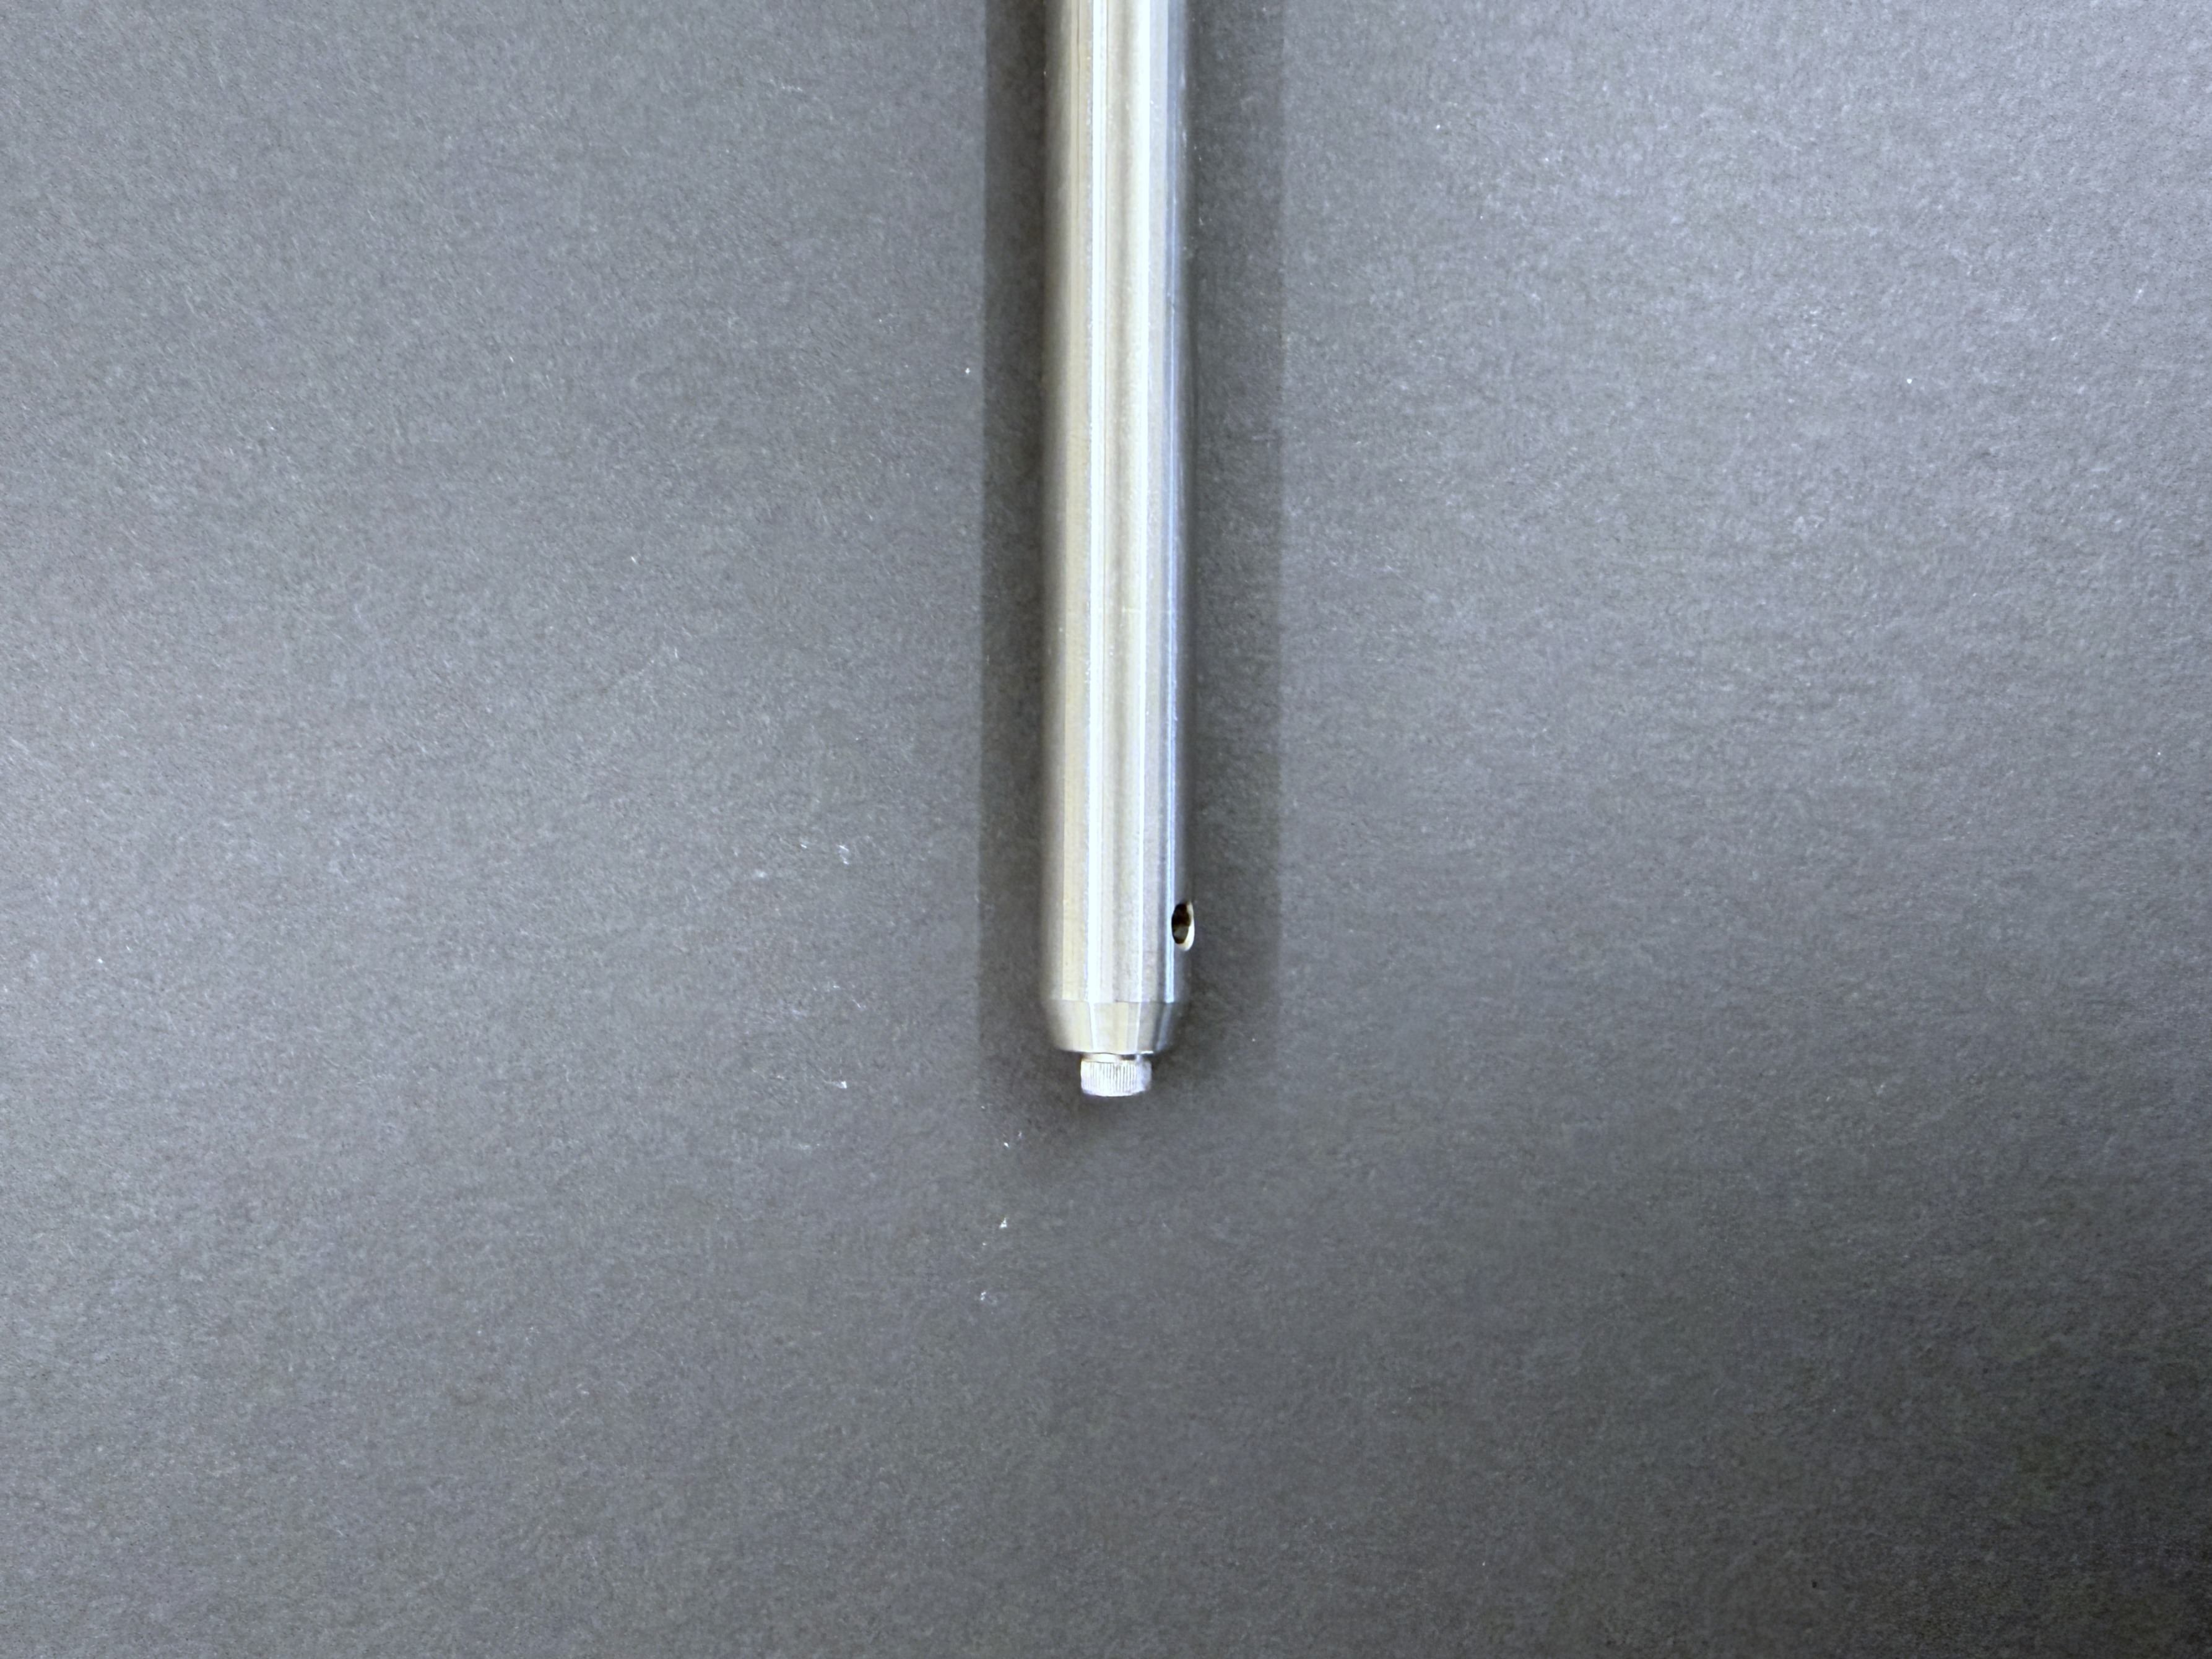
\includegraphics[width=6cm]{point_indenter}};
		\node[anchor=north west,inner sep=0] at (6,0) {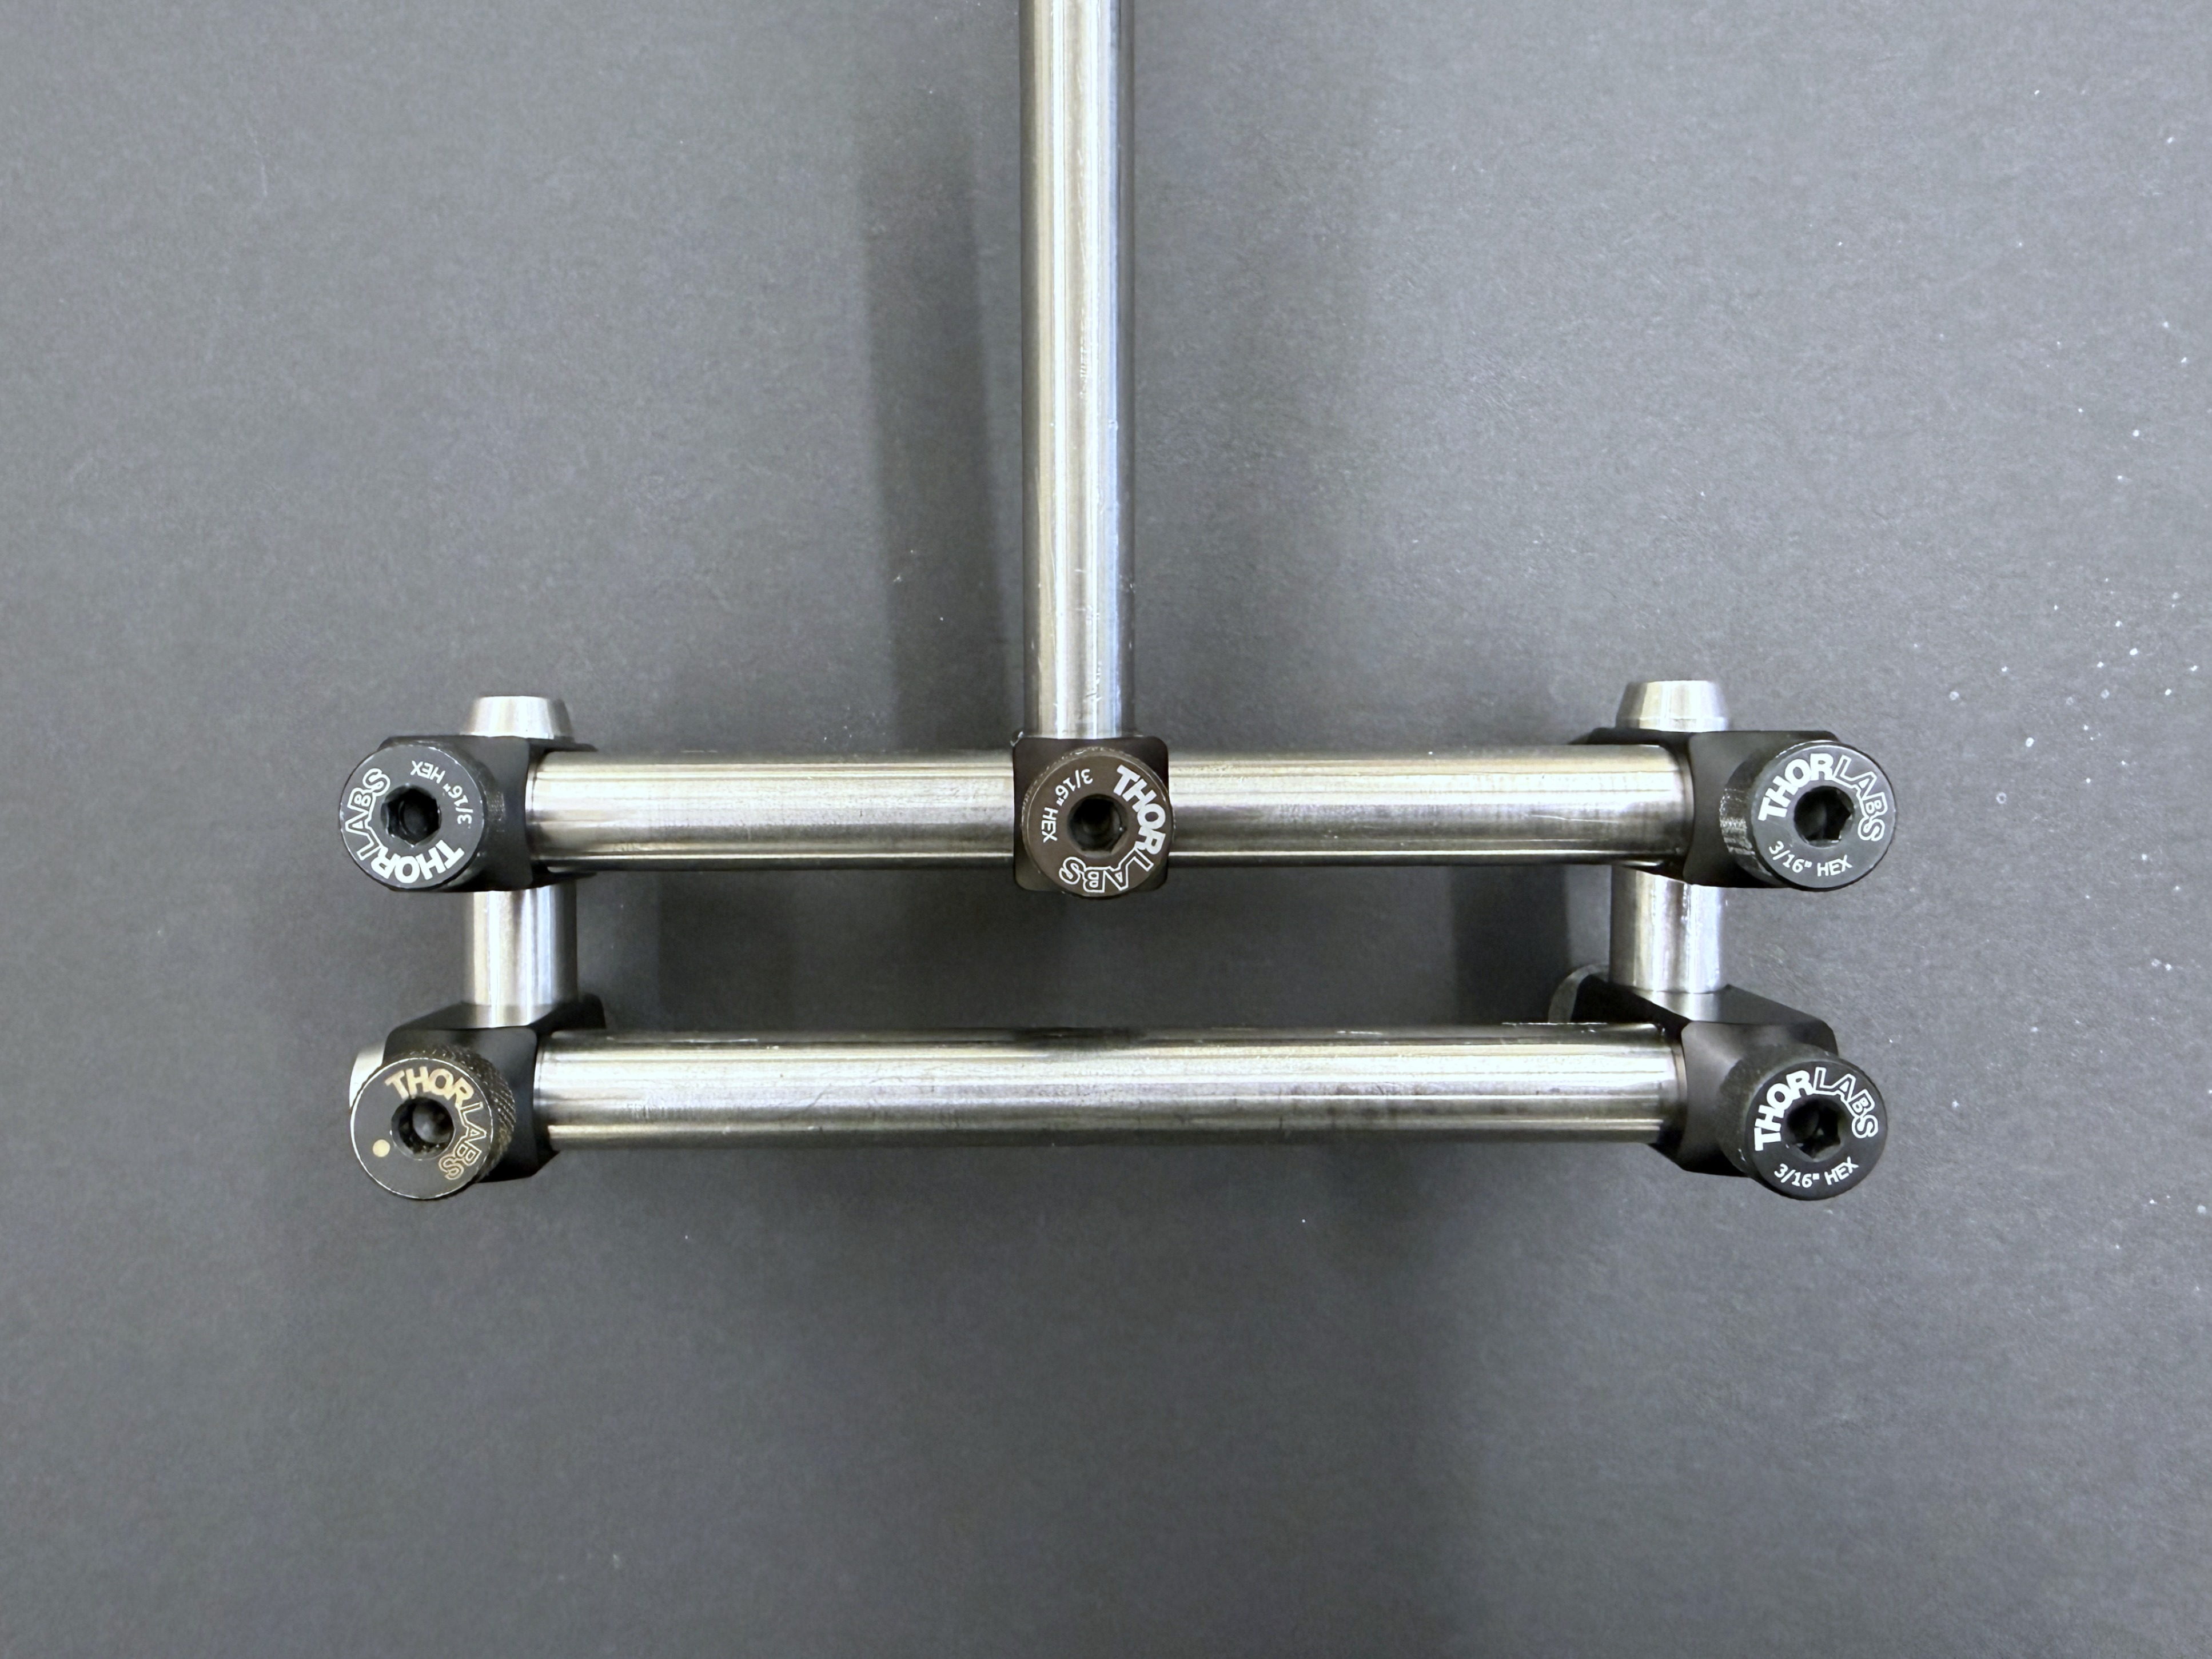
\includegraphics[width=6cm]{cylinder_indenter}};
		
		\node[anchor=north east,inner sep=0] at (6,0) {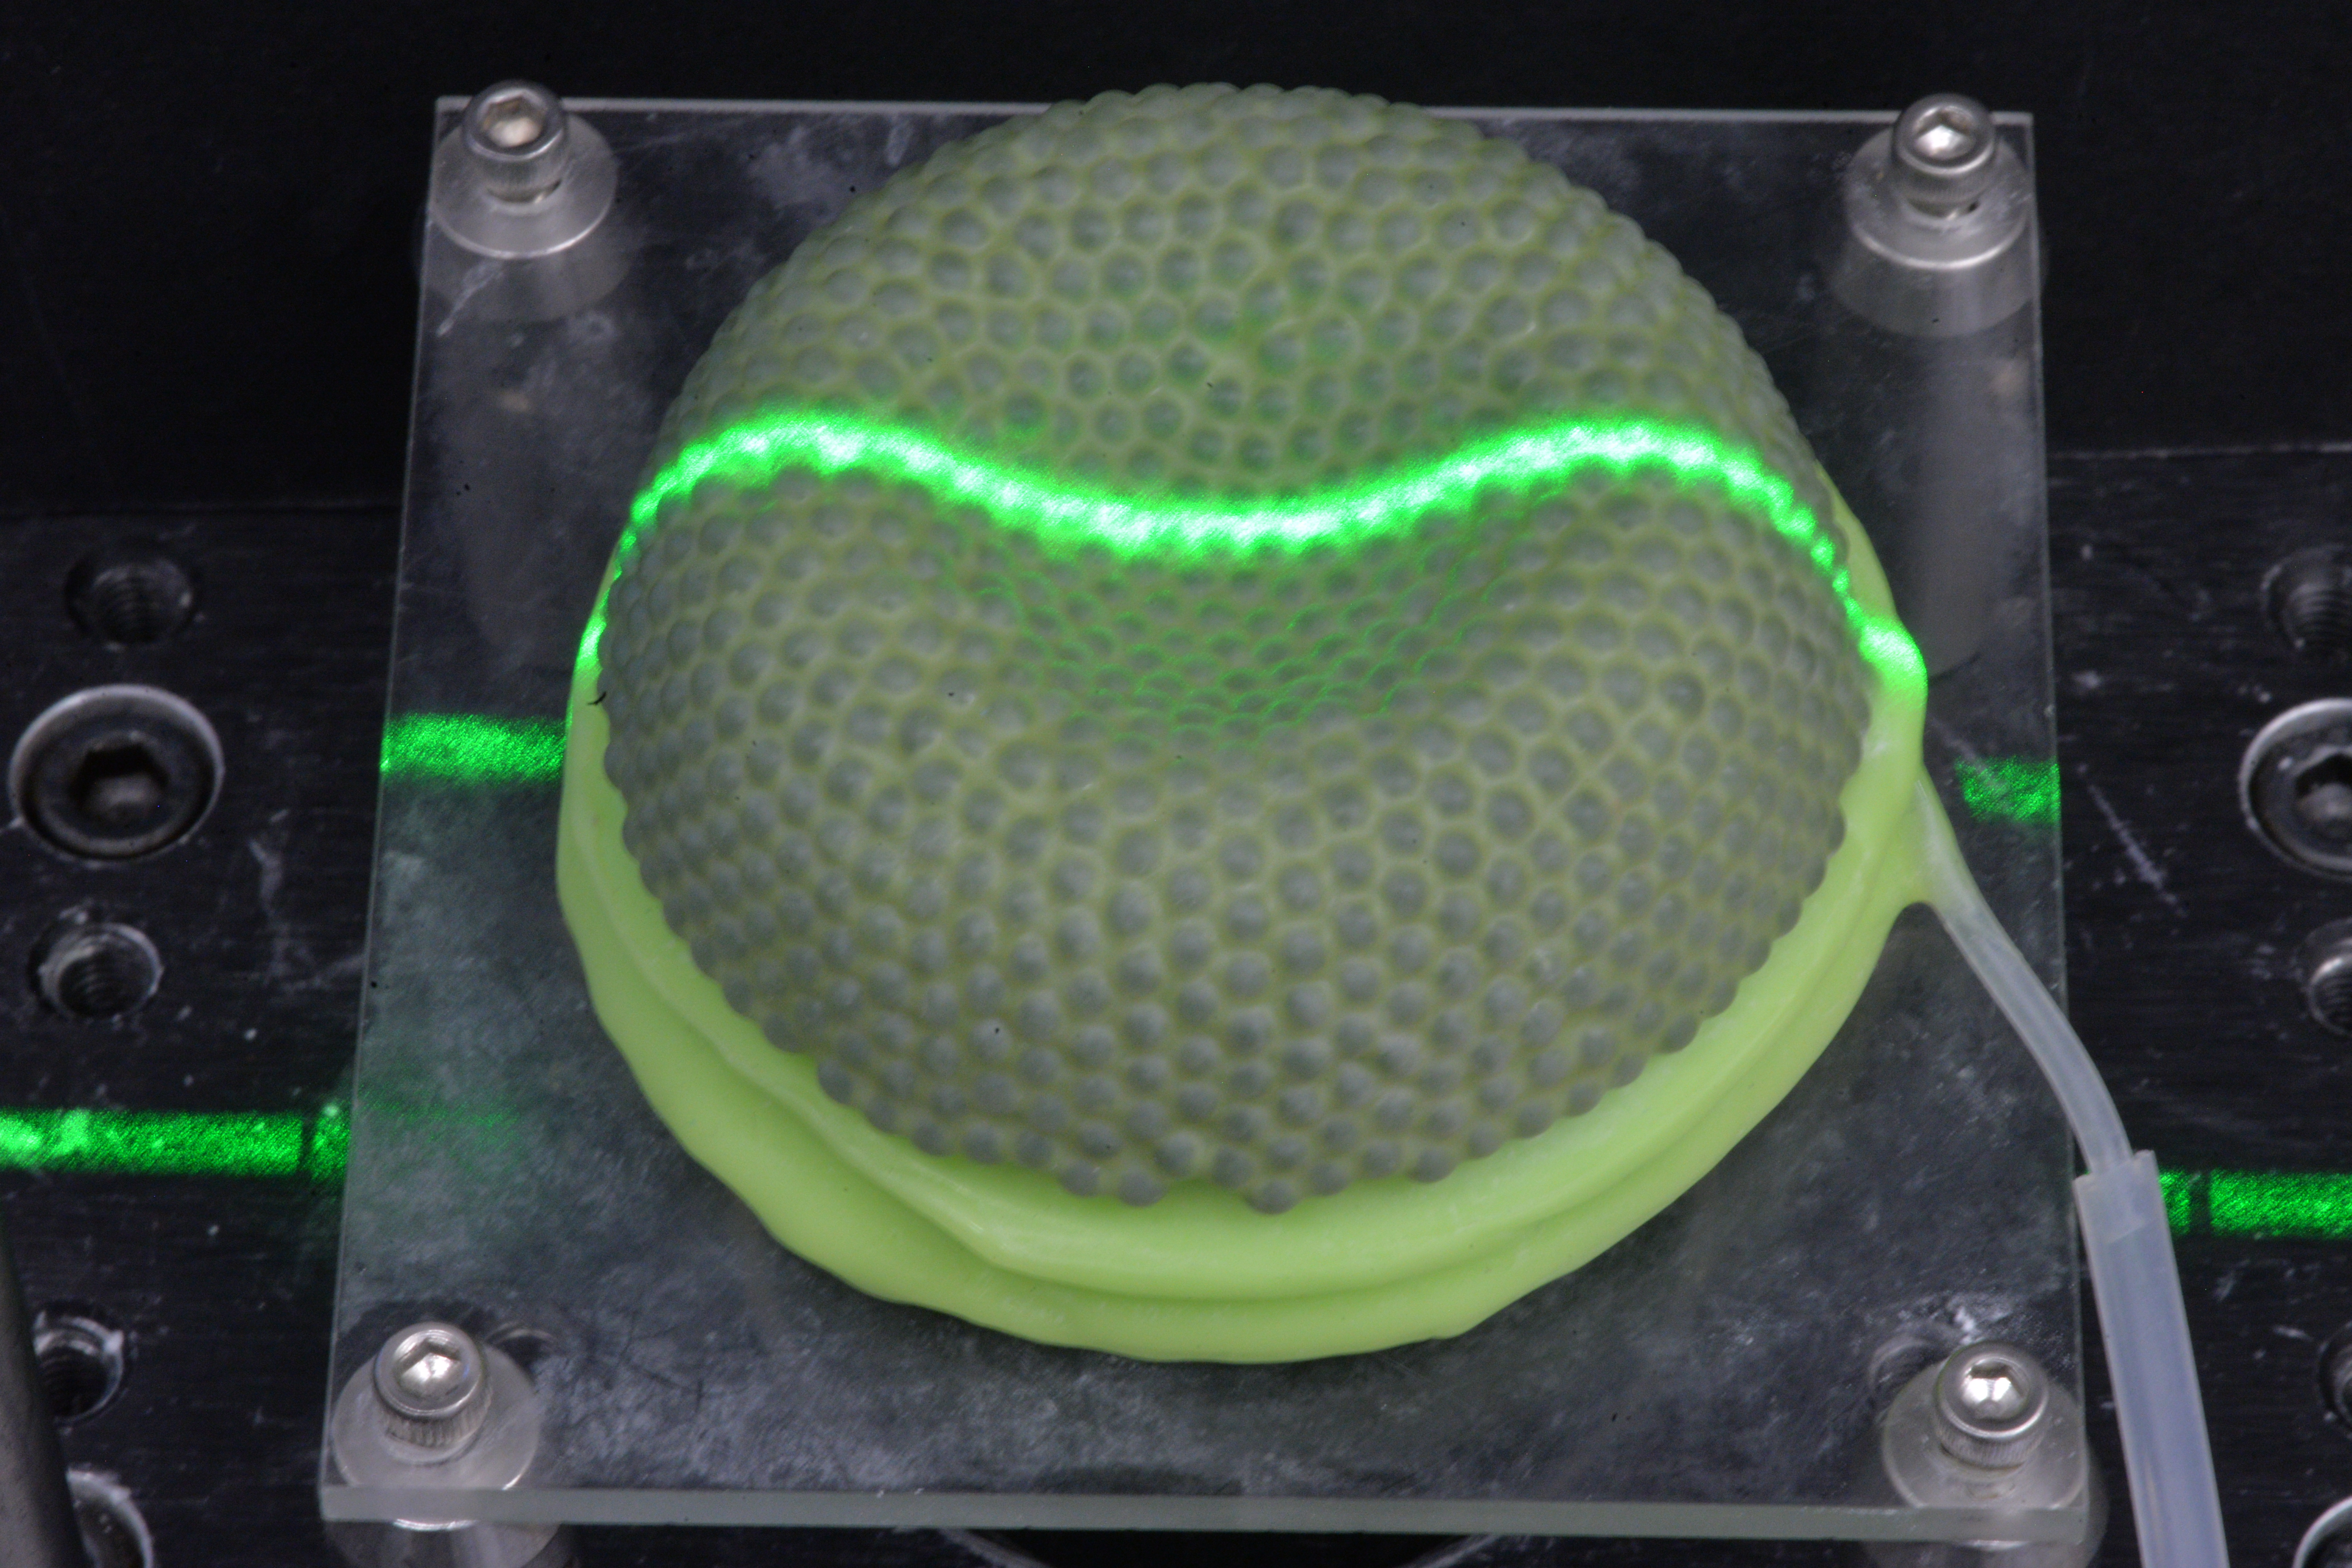
\includegraphics[width=2.25cm]{indent-point}};
		\node[anchor=north east,inner sep=0] at (12,0) {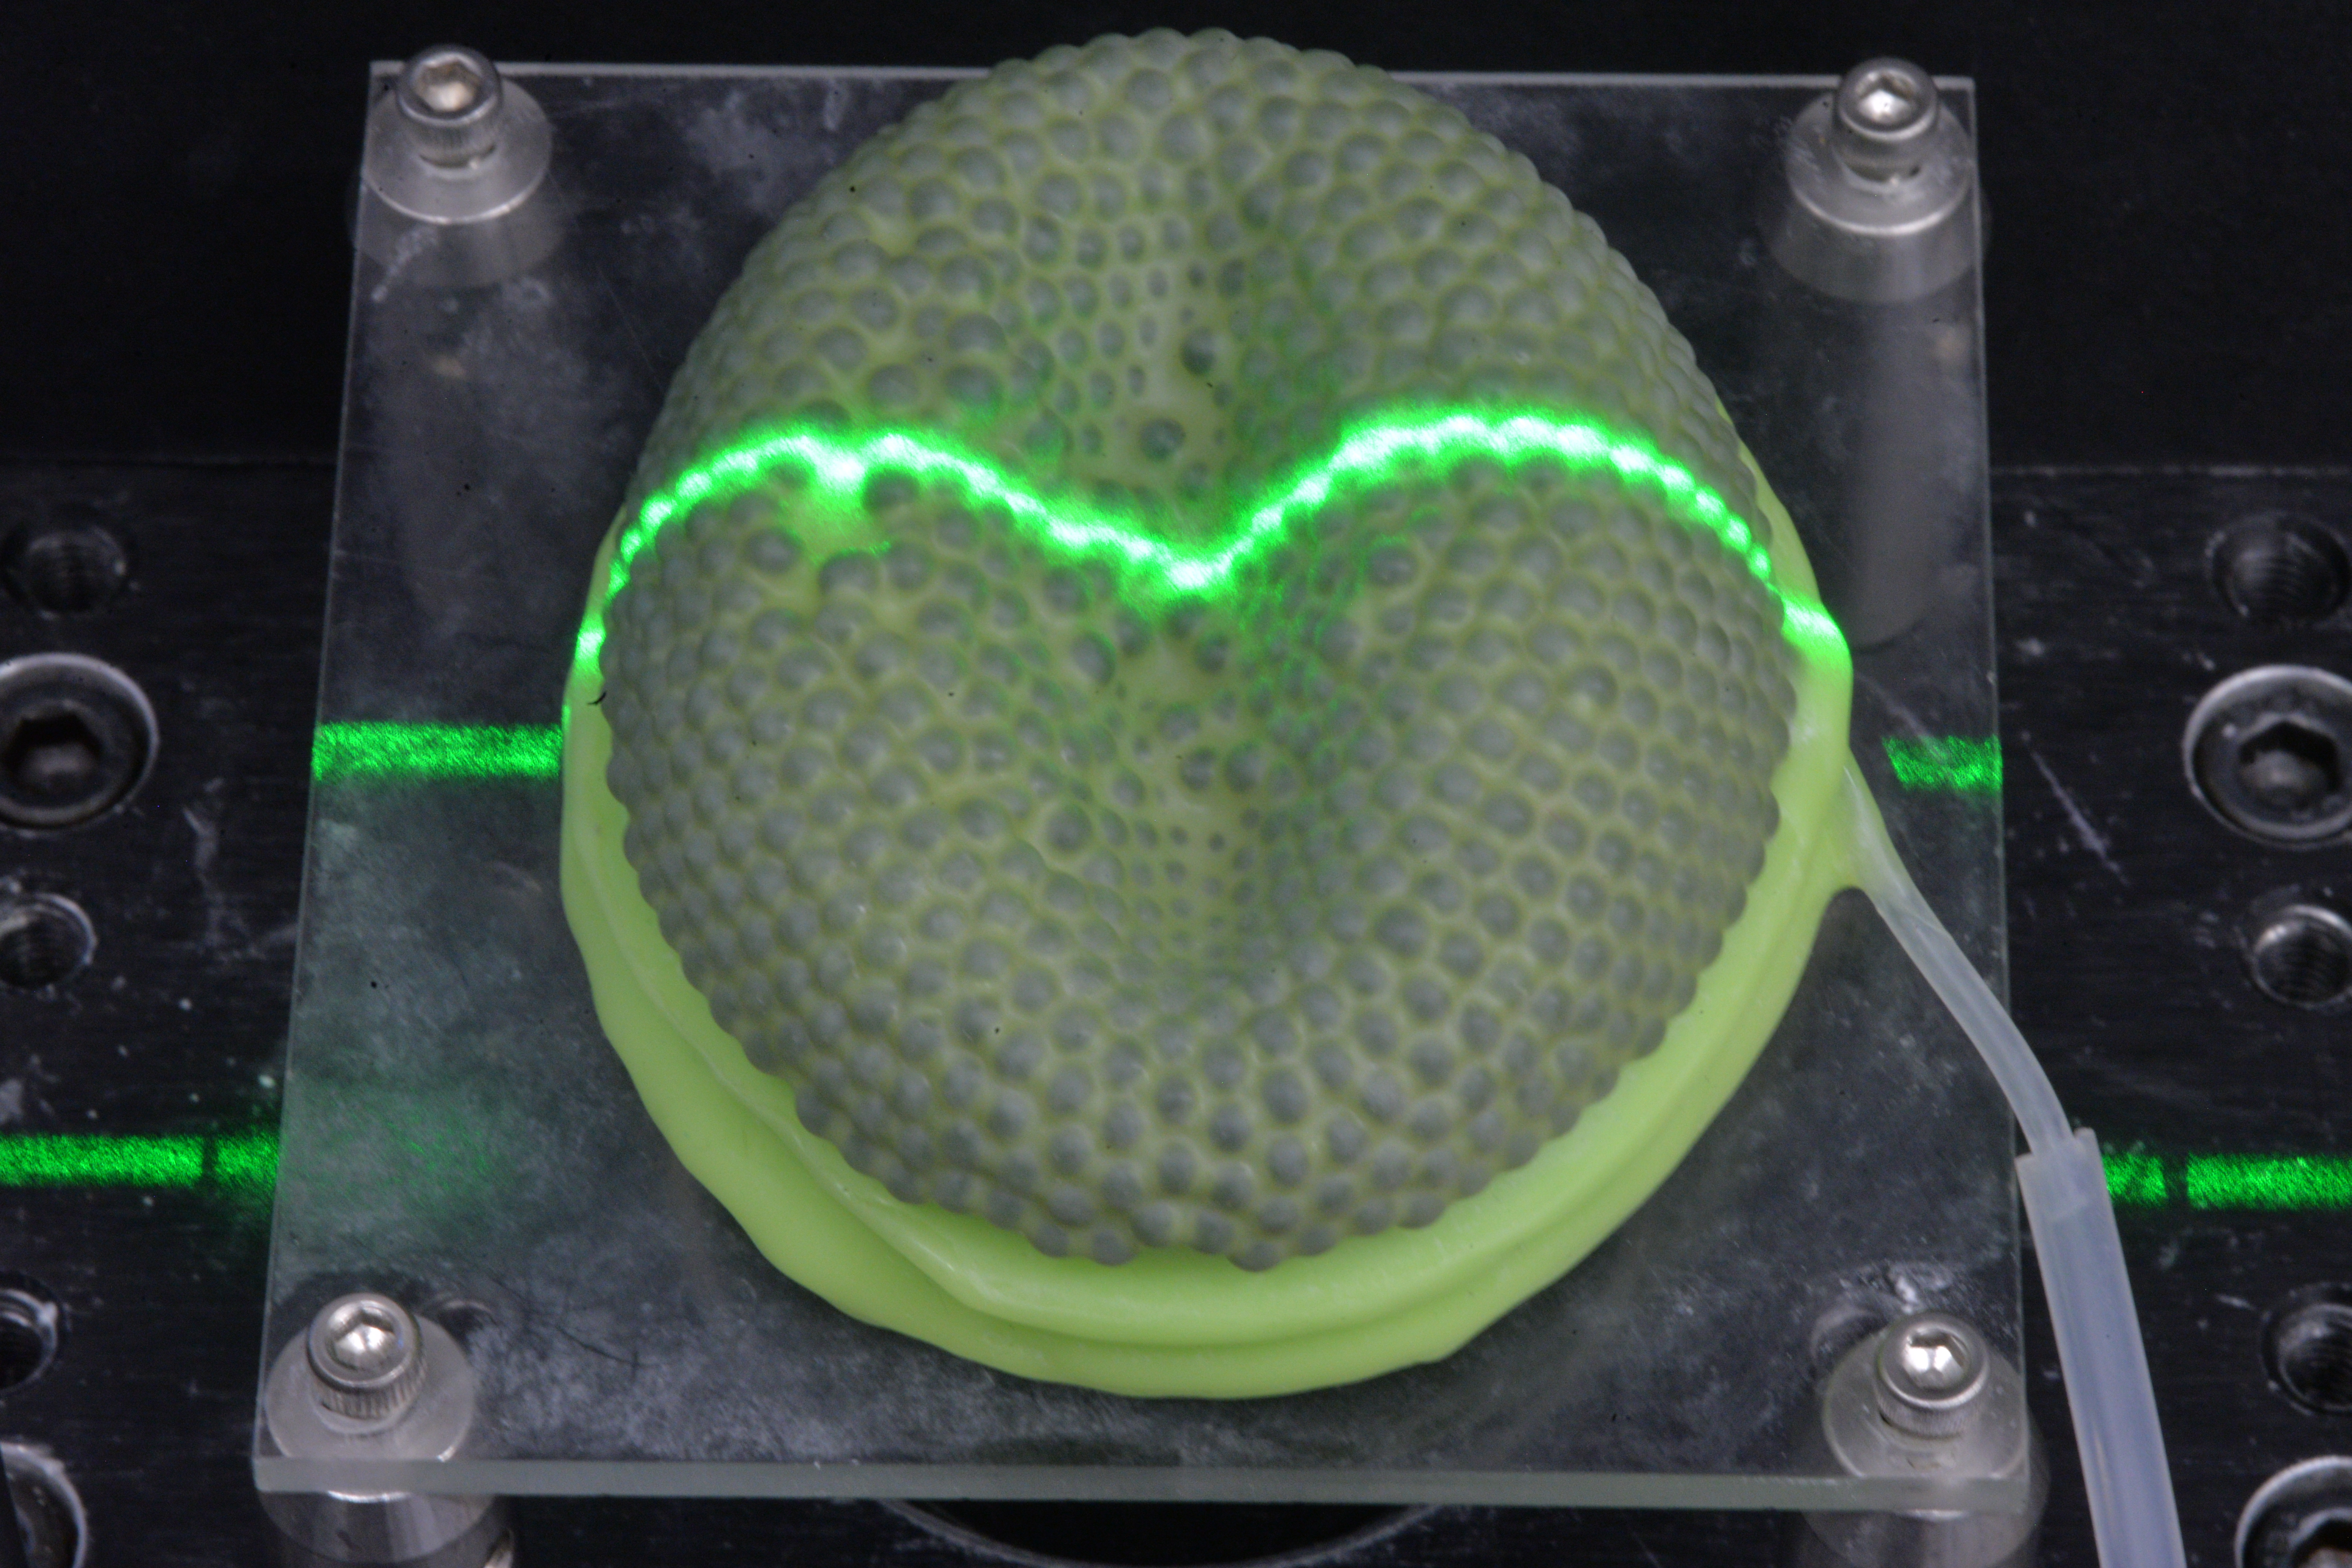
\includegraphics[width=2.25cm]{indent-rod}};

		
		
		
		\node [anchor=south west] at (0.1,-0.75) {\color{white}{$a.$}};
		\node [anchor=south west] at (6.1,-0.75) {\color{white}{$b.$}};
		
		
		\draw [anchor=north east,white,ultra thick,inner sep=0] (4,-4.25) -- (5.6,-4.25);
		\node [anchor=north west] at (3.825,-3.6) {\color{white}{{{20 mm}}}};
		
		 \draw[line width=2pt,-Stealth,white]        (3.05,-3.25)   -- (3.05,-4.25);
		\node at (2.65,-3.75) {\color{white}{{{$\delta$}}}};
		
		
		\draw [anchor=north east,white,ultra thick,inner sep=0] (10,-4.25) -- (11.6,-4.25);
		\node [anchor=north west] at (9.825,-3.6) {\color{white}{{{60 mm}}}};
		
		\draw[line width=2pt,-Stealth,white]        (9.05,-3.25)   -- (9.05,-4.25);
		\node at (8.65,-3.75) {\color{white}{{{$\delta$}}}};
		
		
	\end{tikzpicture}
	
	
\end{document}
